
\chapter{Particle velocimetry of vortices in Bose–Einstein condensates}

    \section{Semiclassical simulations}
    Provide details of how the simulations were performed and the results they gave. Describe method of computing collisions between the classically modelled particles and the condensate, and how the fluorescence imaging was simulated. Present results and discuss experimental feasibility.

    \section{Sisyphus cooling in a magnetic field}
    Describe the scheme for Sisyphus cooling I developed, and show 1D simulation results.

\begin{figure}
\begin{center}
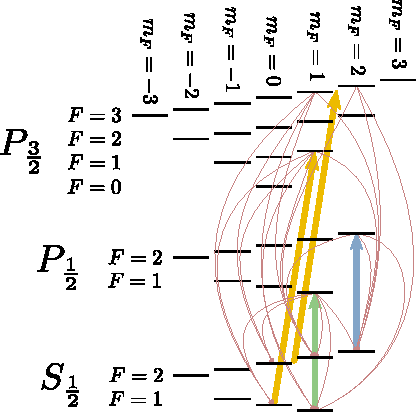
\includegraphics[width=0.65\textwidth]{figures/cooling_full.pdf}
\caption{\label{fig:cooling_full} The full cooling scheme, including repump lasers (yellow), cooling lasers (blue and green), and all possible decay paths (red). The repump beam which is drawn in between two ground and excited states has a frequency equal to the average of those two transitions. }
\end{center}
\end{figure}


\lipsum[1-5]


\begin{figure}
\begin{center}
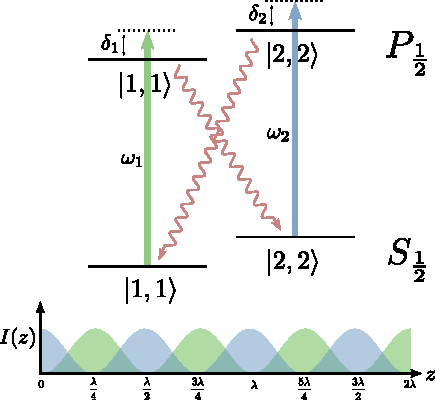
\includegraphics[width=0.65\textwidth]{figures/cooling_simplified.pdf}
\caption{\label{fig:cooling_simplified}An idealised depiction of the cooling scheme, with repump lasers and undesired states not shown. Two lasers on the D$_1$ line are used for cooling, both linearly polarised, and arranged so as to form two interleaved standing waves. Both are blue detuned from the transitions they target, and they differ by about $6.8\,$GHz. This difference means that the alignment of the two standing waves can only be maintained over a distance of about a centimetre.}
\end{center}
\end{figure}

\lipsum[1-5]
